

\section{Somaïr}
Dans cette partie, nous allons tout particulièrement nous intéresser au fonctionnement de Somaïr, la mine à ciel ouvert d'Orano au Niger, car c'est la qu'est déployé l'outil CanOp et qui me faut comprendre le fonctionement pour donner des suggestions cohérentes.%jv avec sopamine%citer pourcentage
\subsection{L'exploration}

Le cycle de vie de la mine commence d'abord par toruver un gisment exploitable. Le service Geoscience de la mine en est reponsable. Il y a une petite équipe d'expert qui en analysant les données géologiques et geopolitique vont déterminer où on peut mener un projet d'exploitation. Cela peut etre une extenstion sur un gisment connu On va ensuite enregistre des "claims" auprès du gouvernement local pour avoir le droit d'exporer le sous-sol. Un projet d'exporation peut prendre 2 formes~:
\begin{description}
    \item[L'exploration "grass roots"] Dans ce type d'exploration, nous avons aucune inormation sur la zone et il faut donc etablire les carte geologique et mener un raisonement sur quel processus geologique aurait pu concentrer l'uranium a un endroit donné. Nous pouvons ensuite faire des forages\footnote{Comme l'uranium est radiactif, nous pouvons approximer la presence de radioactiviter a la precense d'uranium} pour verifier nos hypothèses. %\footnote{environ \sfrac{3}{4} des forage ne donne aucun resulatat}
    \item[L'exploration "brown fields"] Comme cela fait de nombreuse année que l'on exploite de l'uranium, certain zone sont deja eu des forage ou sont a proximité de zone exploité. On vas donc reprendre les données brute relative a la zone et chercher quel assuption on etait fait par le passer et si les personne precedant on neglige quelque chose.
\end{description}
L'etape d'exploration est complique car plus un gisement est concentrer alors plus il auras tendance a etre petit et donc plus il est difficile a trouver.

Une fois le gisement trouvé, on vas multiplier les forages pour comprendre la forme et la repartition du gisement. Une fois que l'on a ateint un degres de confiance suiffisant, le gisment est dit "ressource" et on peut alors passer a l'etape d'extraction.







\subsection{L'extraction}
\label{ssec_extraction}
A Somaïr, la profondeur du gisement, sa forme, la geographie du site et la teneur on fait que le methode d'extraction la plus rentable est une mine a ciel ouvert.

On comence d'abord par decouvire le gisment, c'est a dire d'enlever les 50 à 70m de roche au dessus du gisment. Cette roche serait utiliser pour reboucher la mine quand elle arriveras en fin de vie.

L'exctraction de l'uranium se fait par "tir". Un tir est une explosion controler qui va briser la roche en morceau plus petit. On delimiter une zone de 50*50*6m dans lequelle on perce des trous tout les 5m. On utilise d'abors ces trous pour faire une mesure de radiometrie qui vas nous permetre d'etablire un plan de trie avant de leus remplir d'explosifs. Une fois les explosifs detoné, un Aide Prospecteur (AP) va mesurer la teneur en uranium de chaque slab\footnote{Un slab est un morceau de roche de 2.5*2.5*0.5m. C'est l'uniter de base de la mine} pour le classer en fonction de sa teneur en uranium.


\subsection{Classification des slabs}
\label{ssec_classification}
\begin{figure}

    \begin{subfigure}[t]{0.4\textwidth}
        \centering
        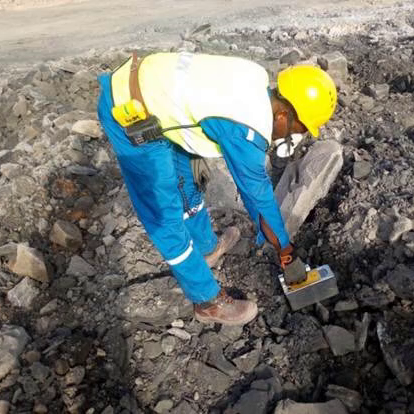
\includegraphics[height=0.3\paperwidth]{photo/Travail_geiger.png}
        \caption{Photo d'un operateur utilisant un compteur Geiger Müller pour mesurer la teneur en uranium d'un slab}
        \label{fig_AP_geiger}
    \end{subfigure}
    \begin{subfigure}[t]{0.6\textwidth}
        \centering
        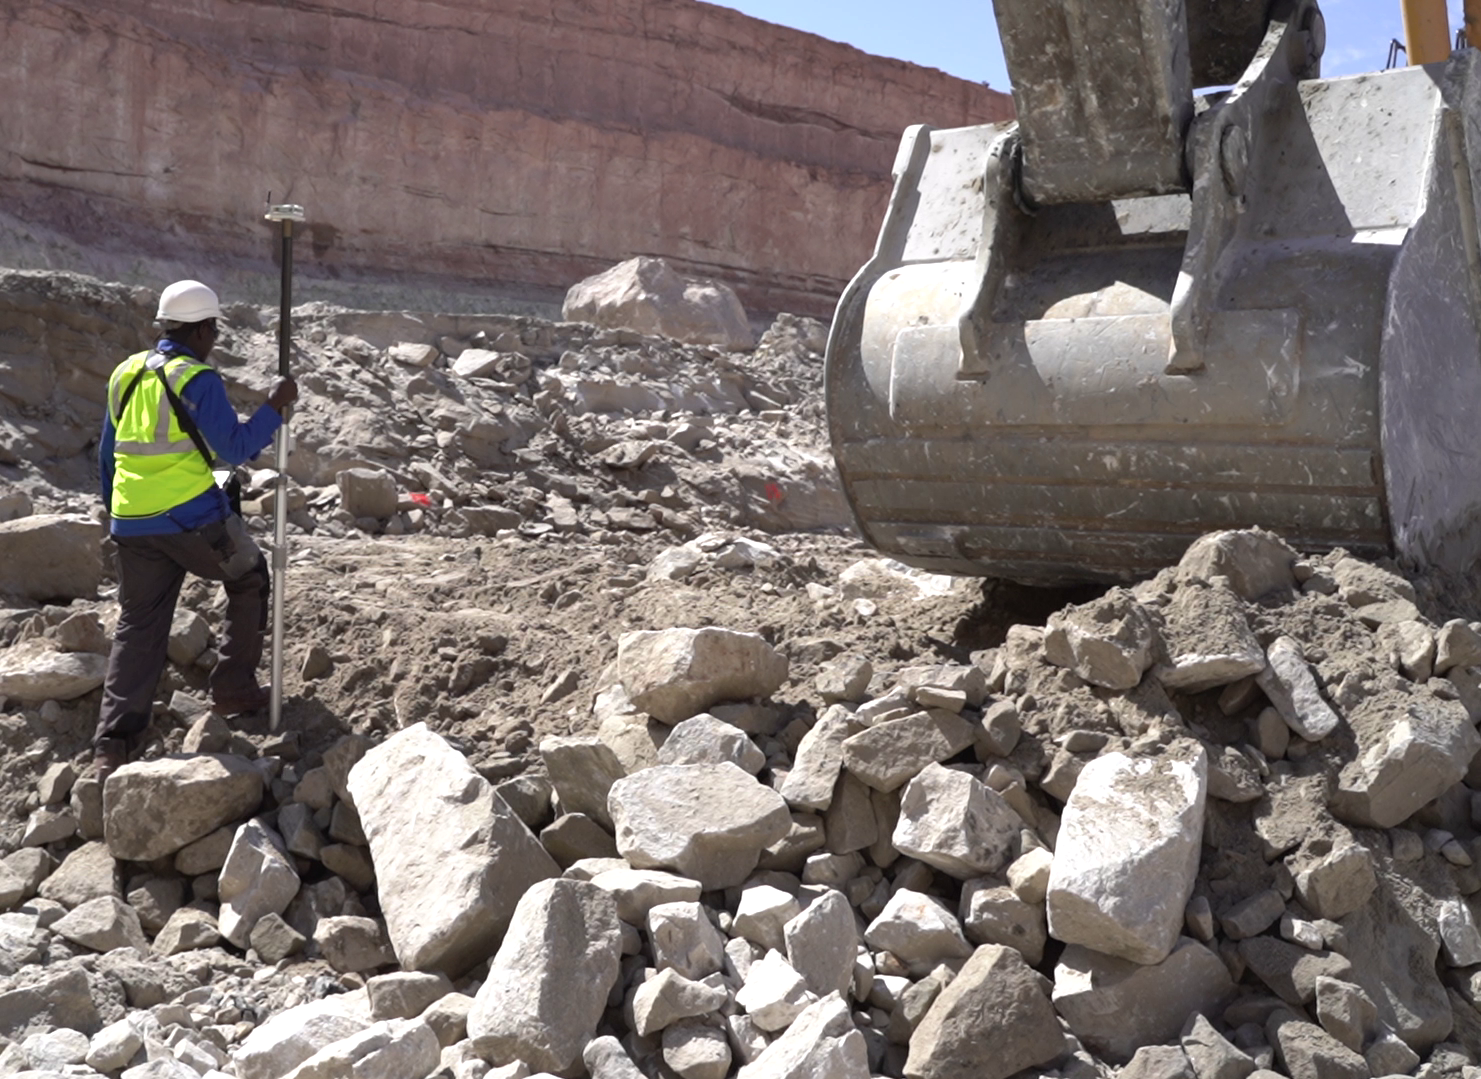
\includegraphics[height=0.3\paperwidth]{photo/CanOp_utilisation.png}
        \caption{Photo d'un operateur utilisant la CanOp pour mesurer la teneur en uranium d'un slab. Il porte une tablette pour voir les mesure et sa position en temps reel}
        \label{fig_AP_CanOp}
    \end{subfigure}
    \caption{Photo d'AP utilisant un compteur Geiger Müller et la CanOp}
\end{figure}
Pour savoir comment traiter ces slabs  après extraction, nous les catégorisons en 7~classes de M0 à M6 en fonction de leur teneur en uranium. Les slabs~M0 sont dites stériles, car elle contient tellement peu d'uranium que l'on ne souhaite pas les traiter. Les classes~M1 et M2 subissent un traitement que l'on dit statique, car c'est slab sont empiler et l’on attend que l'uranium descend par gravité jusqu'un bas. Enfin les slabs de classe supérieure reçoivent un traitement dynamique où en fonction de leur classe elles seront dissoutes avec plus ou moins d'acide selon leurs classes. Il est donc important de bien classer les slabs, car sinon, soit on gaspille  de l'acide ou alors il reste des l'uranium non extrait dans notre refus.
%TODO:mistakes
Avant, pour classer une slab, un Aide Prospecteur (AP) utiliser un compteur Geiger Müller en se penchant pour obtenir des mesures a plusieurs points sur le slab. Il était donc pénible de se pencher en permanence et donc en 2018 a été lancer le projet CanOp pour réduire la pénibilité de la tache et optimiser le tri du minerai.
